\subsection{V2a}
\label{sec:E2-V2a}
\renewcommand{\Vs}{V2a}
In this experiment, we have a camera recording of traffic, but the view is obstructed by a significant obstacle,
disposing any object detection system of the capability to capture targets. To simulate this situation, we
artificially
add a road crossing the main highway line in the video \textit{V2}. Although it is evident that the added road does
not belong to the scene, its color characteristics closely resemble those of the natural highway line. Furthermore,
the video playback frame rate is decreased to 10 fps.

\subsection{V2a -- GM-PHD with the dynamic detection probability}
Based on the prior experiments, it is deemed unproductive to assess the GM-PHD filter under the constant detection
probability. If the adapted GM-PHD filter demonstrates the capability to track objects even in areas lacking measurements, the forthcoming experiment, designated as setting \textit{S1}, is suggested.

\subsubsection{S1 -- YOLO + YOLO}
\renewcommand{\Set}{S1}
This experiment employs settings \textit{S1} on the video \textit{V2}, which includes an additional obstacle.
The parameter settings are shown in Table \ref{tab:\Ex-\Vs-\Set}.
\begin{table}[H]
    \centering
    \begin{tabular}{|c|c|c|c|c|c|c|c|c|}
        \hline
        $P_{D,k}(x)$ & $P$ & $\sigma_{\upsilon}$ & $\sigma_{\epsilon}$ & $T_H$ & $T_d$ & $T_p$ & $T_l$ & $T_{YOLO}$ \\ \noalign{\hrule
        height 1.5pt}
        0.3 & $\diag(40,40,40,40)$ & 0.04 & 120 & 0.5 & 3 & 0.1 & 0.001 & 0.3\\
        \hline
    \end{tabular}
    \caption{The parameter settings for Experiment {\Ex-\Vs-\Set} with the dynamic detection probability.}
    \label{tab:\Ex-\Vs-\Set}
\end{table}

In Figure \ref{fig:\Ex-\Vs-\Set} we can see the tracking performance of the GM-PHD filter with settings \textit{S1}
on the traffic situation with an added obstacle. For this experiment, two additional bounding boxes are displayed.
The blue bbox represents the place, the target has been lastly detected in. The black bbox is the moving bbox from Equation \eqref{eq:mphd_bbox_shift}. The color characterics of the scene given by these two bounding boxes are compared to calculate $p_{H,k}$ in \eqref{eq:mphd_recursion_update_intesity_misdetect_pH}.
\begin{itemize}
    \item \textbf{\ref{fig:\Ex-\Vs-\Set:01}:} The tracking starts with the frame no. 47. There are two cars next to each
    other. At this moment, the cars are coming close to the obstacle.
    \item \textbf{\ref{fig:\Ex-\Vs-\Set:02}:} The targets are obscured and remain undetected, with their state labeled as \textit{hidden}.
    \item \textbf{\ref{fig:\Ex-\Vs-\Set:03}:} Given the characteristics of the scene, the targets' positions lag slightly behind their true positions.
    \item \textbf{\ref{fig:\Ex-\Vs-\Set:04}:} The cars are detected again and, due to the large covariance, the
    targets get their measurements.
    \item \textbf{\ref{fig:\Ex-\Vs-\Set:05}:} Nevertheless, one false target still falls behind the true targets.
    \item \textbf{\ref{fig:\Ex-\Vs-\Set:06}:} Even though the true targets continue in their path with correct measurements, the false target persists.
    \item \textbf{\ref{fig:\Ex-\Vs-\Set:07}:} Due to the similar characteristics of the added road with the actual highway road, the false target is considered as hidden.
    \item \textbf{\ref{fig:\Ex-\Vs-\Set:08}:} Finally the false target is removed, not due to exceeding the lowered threshold $T_l$, but due to the change of its state to \textit{dead}.
\end{itemize}

In this experiment, we demonstrated that with the GM-PHD filter with the dynamic detection probability it is possible
to overcome an obstacle blocking the view of the camera. However, another problem arises. If the obstacle has similar color characteristics as the background around the target, the predicted false target survives for too long.
\begin{figure}[H]
    \centering
    \begin{subfigure}{0.48\textwidth}
        \centering
        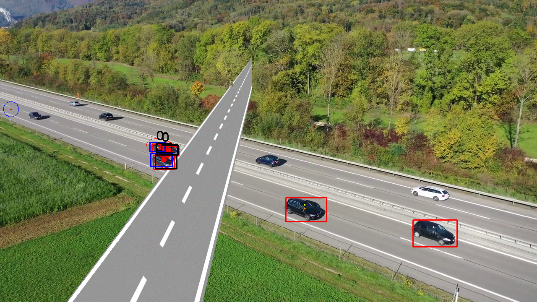
\includegraphics[width=\linewidth]{../../../experiments/\Ex/\Vs/YOLO/47}
        \caption{Frame number: 47.}
        \label{fig:\Ex-\Vs-\Set:01}
    \end{subfigure}
    \begin{subfigure}{0.48\textwidth}
        \centering
        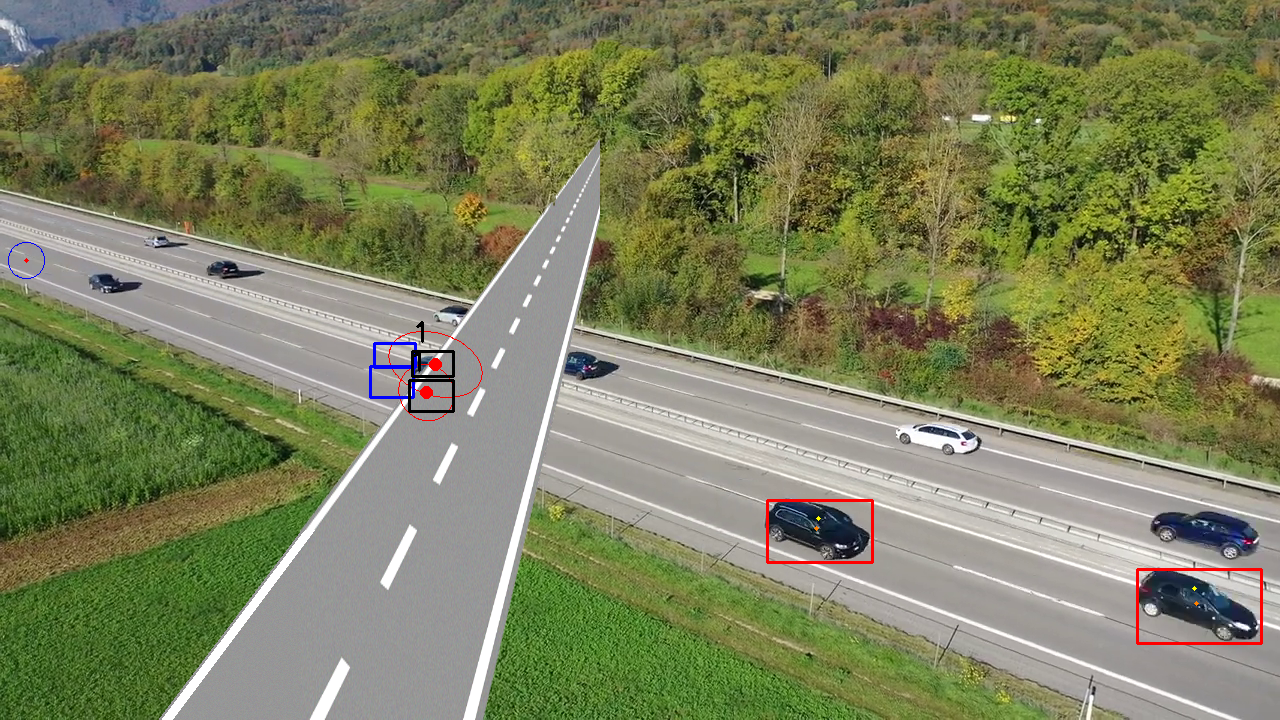
\includegraphics[width=\linewidth]{../../../experiments/\Ex/\Vs/YOLO/50}
        \caption{Frame number: 50.}
        \label{fig:\Ex-\Vs-\Set:02}
    \end{subfigure}
    \\
    \begin{subfigure}{0.48\textwidth}
        \centering
        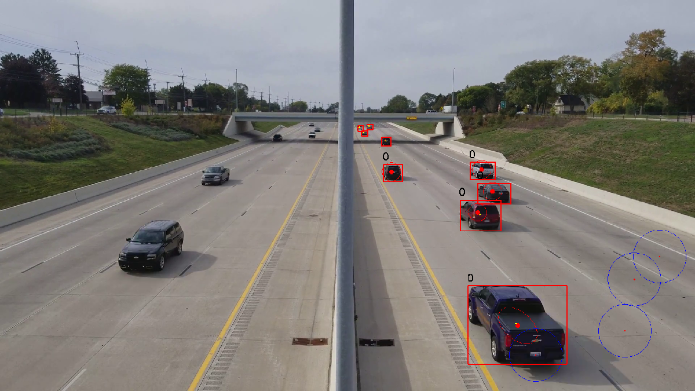
\includegraphics[width=\linewidth]{../../../experiments/\Ex/\Vs/YOLO/54}
        \caption{Frame number: 54.}
        \label{fig:\Ex-\Vs-\Set:03}
    \end{subfigure}
    \begin{subfigure}{0.48\textwidth}
        \centering
        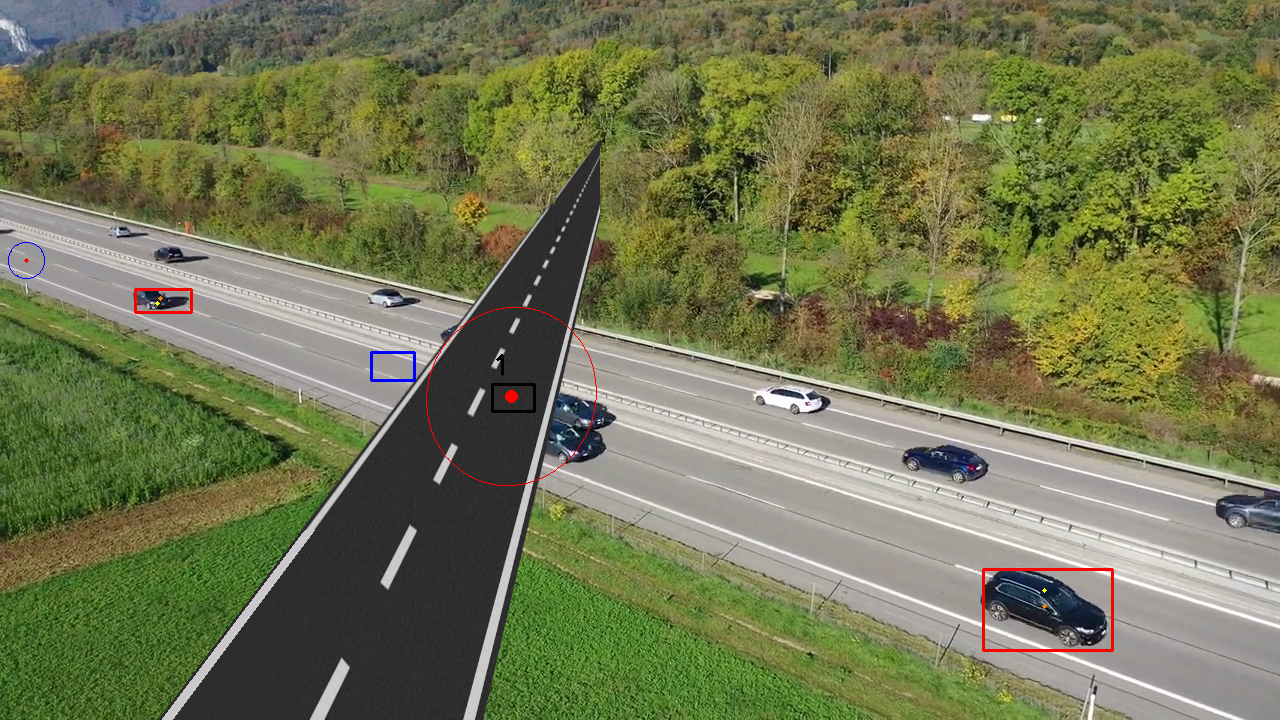
\includegraphics[width=\linewidth]{../../../experiments/\Ex/\Vs/YOLO/56}
        \caption{Frame number: 56.}
        \label{fig:\Ex-\Vs-\Set:04}
    \end{subfigure}
    \\
    \begin{subfigure}{0.48\textwidth}
        \centering
        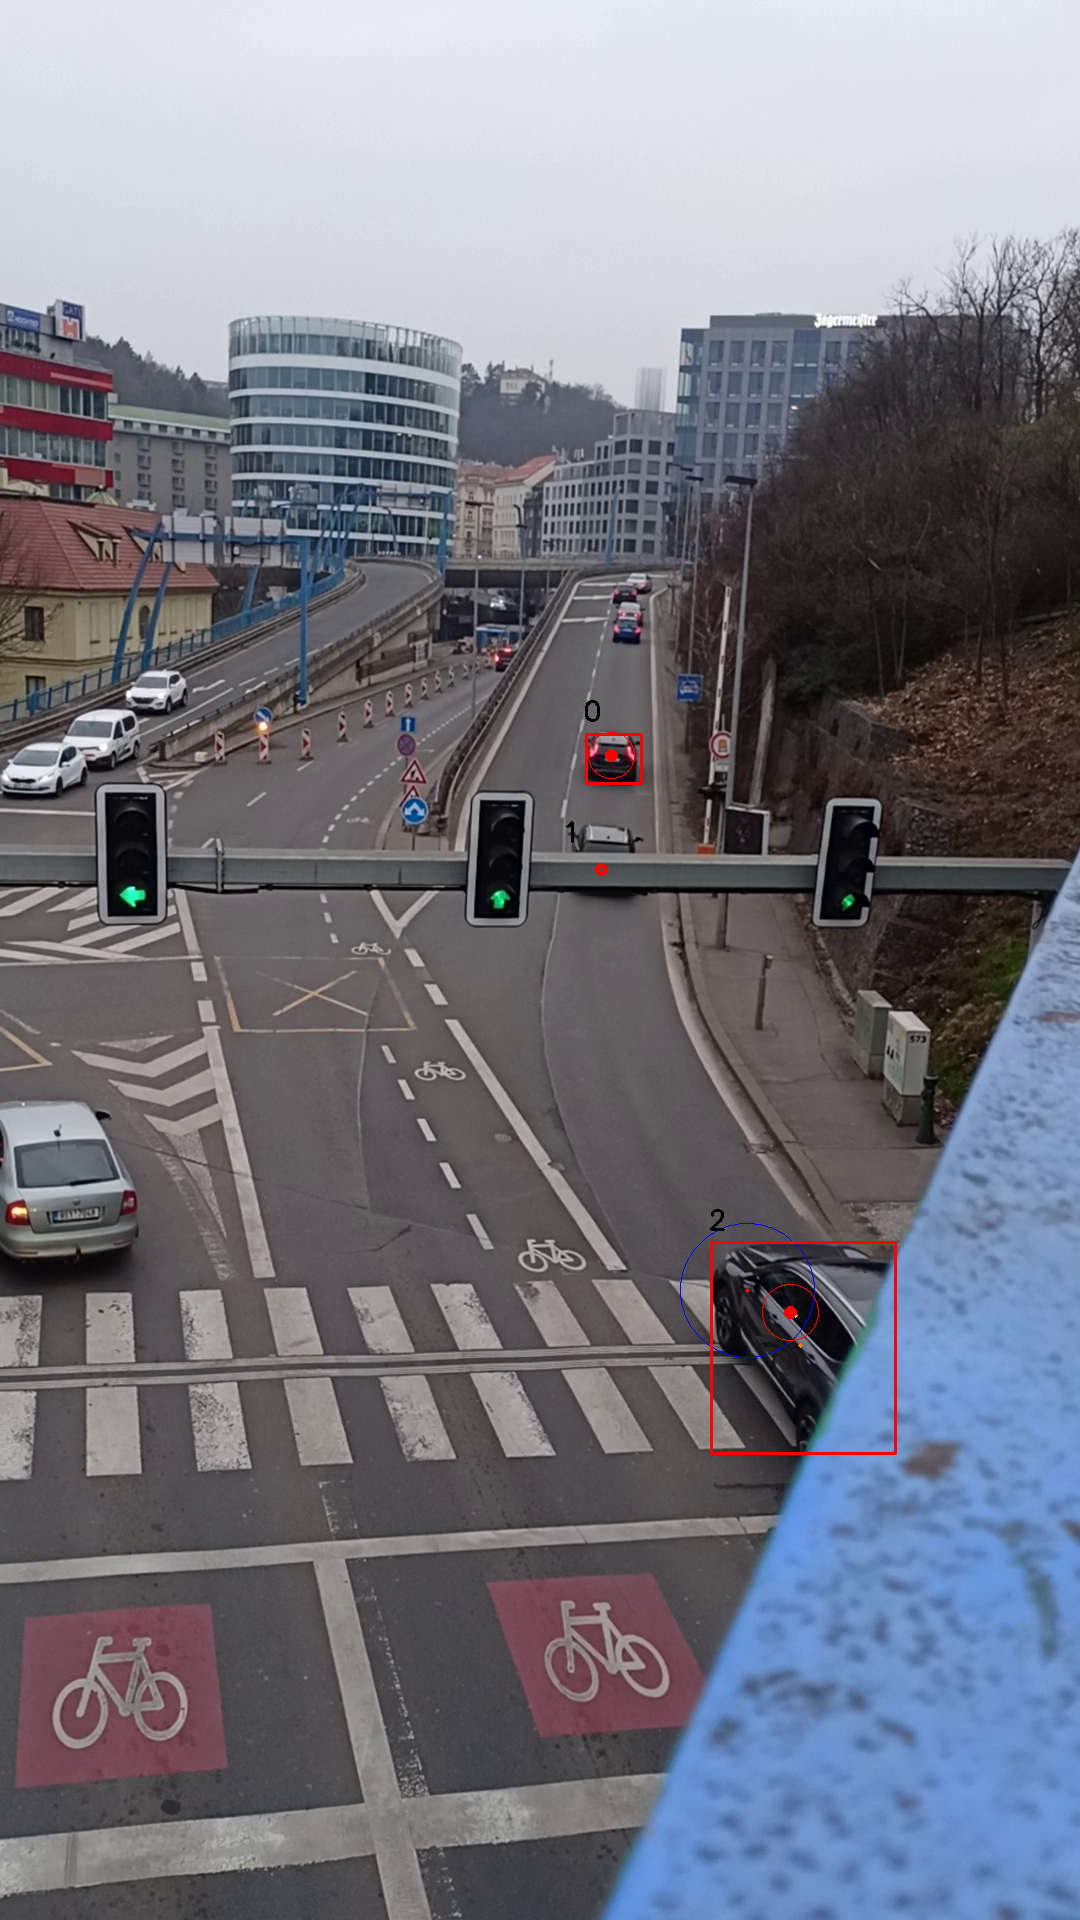
\includegraphics[width=\linewidth]{../../../experiments/\Ex/\Vs/YOLO/57}
        \caption{Frame number: 57.}
        \label{fig:\Ex-\Vs-\Set:05}
    \end{subfigure}
    \begin{subfigure}{0.48\textwidth}
        \centering
        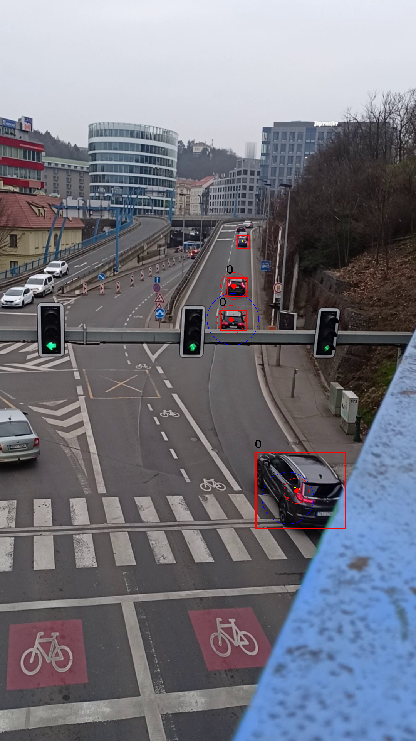
\includegraphics[width=\linewidth]{../../../experiments/\Ex/\Vs/YOLO/60}
        \caption{Frame number: 60.}
        \label{fig:\Ex-\Vs-\Set:06}
    \end{subfigure}
    \\
    \begin{subfigure}{0.48\textwidth}
        \centering
        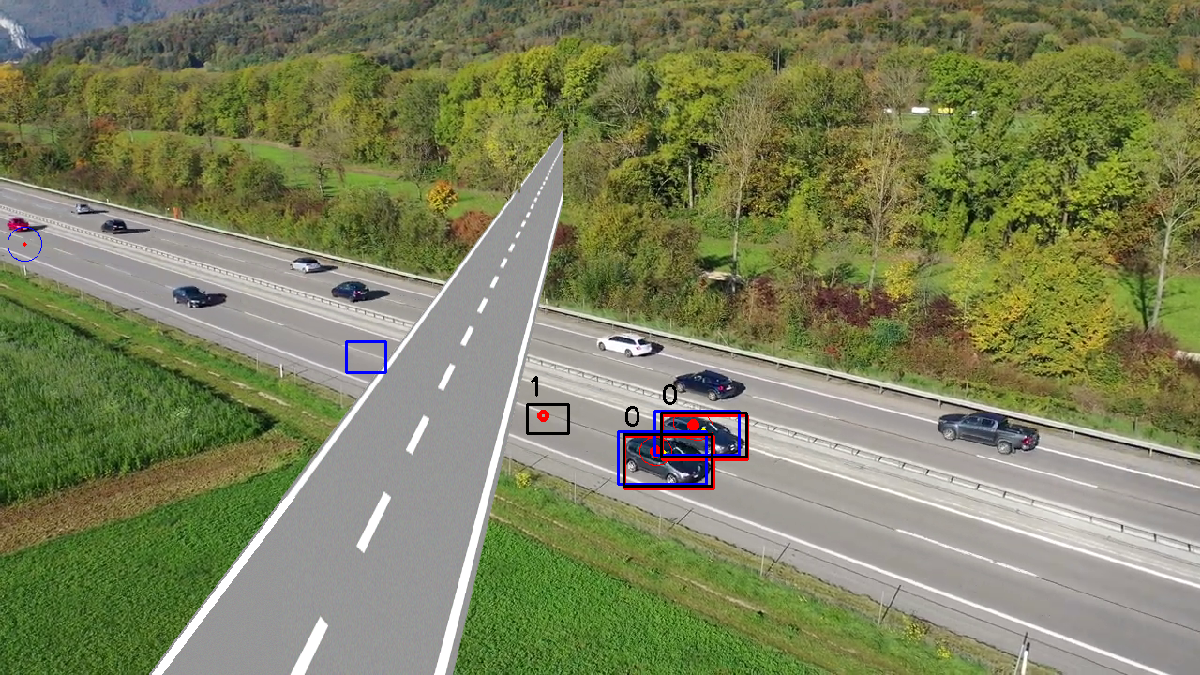
\includegraphics[width=\linewidth]{../../../experiments/\Ex/\Vs/YOLO/62}
        \caption{Frame number: 62.}
        \label{fig:\Ex-\Vs-\Set:07}
    \end{subfigure}
    \begin{subfigure}{0.48\textwidth}
        \centering
        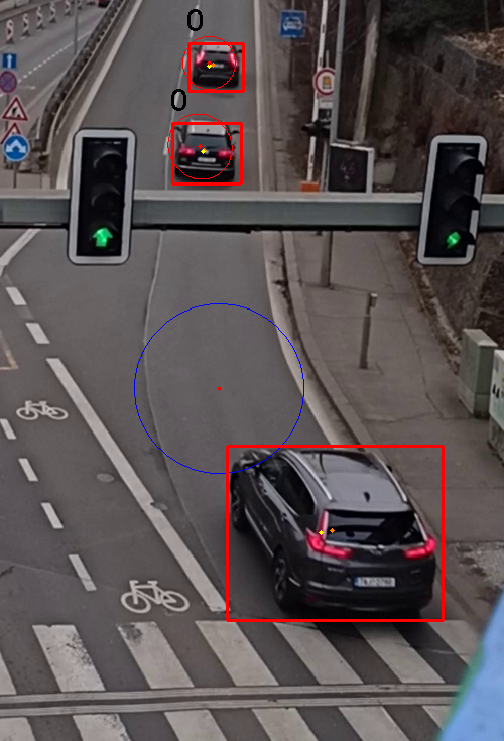
\includegraphics[width=\linewidth]{../../../experiments/\Ex/\Vs/YOLO/63}
        \caption{Frame number: 63.}
        \label{fig:\Ex-\Vs-\Set:08}
    \end{subfigure}
    \caption{Image sequence of the tracked objects using the GM-PHD filter with the dynamic detection probability and
    YOLO only.}
    \label{fig:\Ex-\Vs-\Set}
\end{figure}

